% =====================================================================
%  Do neutron-star glitches keep time?
%  A pre-registered, measurement-aware test of the vortex-creep
%  waiting-time prediction
%
%  Builds with the MNRAS class (mnras.cls, fleqn, usenatbib) when it is
%  available, and otherwise falls back to a plain article layout with the
%  same content.  Tables tab_sample.tex and tab_beta.tex are generated
%  directly from the frozen result files; figures are the pipeline's own
%  PDF outputs (scripts/10_figures.py).
% =====================================================================
\newif\ifmnras
\IfFileExists{mnras.cls}{\mnrastrue}{\mnrasfalse}
\ifmnras
  \documentclass[fleqn,usenatbib]{mnras}
\else
  \documentclass[10pt,a4paper,twocolumn]{article}
  \usepackage[margin=1.8cm,columnsep=0.7cm]{geometry}
  \usepackage[round,authoryear]{natbib}
  \newenvironment{keywords}{\par\noindent\textbf{Key words:} }{\par}
\fi
\usepackage[T1]{fontenc}
\IfFileExists{newtxtext.sty}{\usepackage{newtxtext,newtxmath}}{\usepackage{mathptmx}}
\usepackage{amsmath,graphicx,booktabs,multirow,array}
\usepackage[hidelinks]{hyperref}
\usepackage{xspace}
\graphicspath{{figures/}{./}}

\newcommand{\dnu}{\Delta\nu/\nu}
\newcommand{\dnud}{\Delta\dot\nu/\dot\nu}
\newcommand{\bhat}{\hat b}
\newcommand{\dhat}{\hat d}
\newcommand{\shat}{\hat\sigma}
\newcommand{\psr}[1]{PSR~#1}
\newcommand{\Smodel}{S1m\xspace}
\newcommand{\mnrasref}[2]{MNRAS, #1, #2}

\ifmnras
  \title[Do glitches keep time?]{Do neutron-star glitches keep time? A
  pre-registered, measurement-aware test of the vortex-creep waiting-time
  prediction}
  \author[D. Bothra]{Deeyan Bothra$^{1}$\thanks{E-mail:
  deeyanbothra10@gmail.com}\\
  $^{1}$Independent researcher, Jaipur, Rajasthan, India}
  \date{Accepted XXX. Received YYY; in original form ZZZ}
  \pubyear{2026}
\else
  \title{\textbf{Do neutron-star glitches keep time?}\\[2pt]
  \large A pre-registered, measurement-aware test of the vortex-creep
  waiting-time prediction}
  \author{Deeyan Bothra\\[2pt]
  \small Independent researcher, Jaipur, Rajasthan, India\\
  \small \texttt{deeyanbothra10@gmail.com}}
  \date{}
\fi

\newcommand{\paperabstract}{The vortex-creep model of pulsar glitches predicts the time to the next
glitch from the fractional steps in spin frequency, $\dnu$, and spin-down
rate, $\dnud$, of the last one (Zhou et al. 2022, equation~48). I test this
within pulsars, using 225 inter-glitch intervals (219 completed, 6
censored) in 21 pulsars from the Jodrell Bank Glitch Catalogue. Two
obstacles arise: the predictor contains the glitch size,
which may set waiting times by itself, and published $\Delta\dot\nu$ values
come from fitting methods that can couple the measurement to the following
interval. I therefore separate a scaling test from a test of the
$\Delta\dot\nu$ coefficient at fixed size, audit how each $\Delta\dot\nu$
was measured, emulate every method on synthetic spin-down histories, and
calibrate all statistics against simulated populations in which the
prediction holds, is absent, is replaced by size alone, or is imitated by
measurement bias. The rules were frozen, with externally recorded
checksums, before any statistic linking glitch properties to observed
waits was computed, and the analysis was run once. Waiting times scale with
the predicted ratio (slope $0.27$, 95 per cent interval $0.20$--$0.34$), and
the spin-down step carries the predicted negative coefficient at fixed size
($-0.26$; $-0.38$ to $-0.13$), which neither size-only nor bias-only
populations reproduce. The unit slope is not recovered, consistent with
attenuation by measurement, and post hoc analyses show that the spin-down
dependence varies between pulsars. An unphysical inertia ratio inferred
for the Crab pulsar is traced to catalogue $\Delta\dot\nu$ values that
include fast transients, which equation~48 excludes.}
\newcommand{\paperkeywords}{stars: neutron -- pulsars: general -- dense matter -- methods: statistical}

\begin{document}
\ifmnras
\label{firstpage}
\pagerange{\pageref{firstpage}--\pageref{lastpage}}
\maketitle
\begin{abstract}\paperabstract\end{abstract}
\begin{keywords}\paperkeywords\end{keywords}
\else
\twocolumn[
\begin{@twocolumnfalse}
\maketitle
\begin{abstract}\paperabstract\end{abstract}
\begin{keywords}\paperkeywords\end{keywords}
\vspace{1.2em}
\end{@twocolumnfalse}]
\fi

% =====================================================================
\section{Introduction}\label{sec:intro}
% =====================================================================
A pulsar glitch is a sudden increase in rotation frequency, usually
accompanied by an increase in the magnitude of the spin-down rate that then
relaxes over days to years \citep{espinoza2011,yu2013,basu2022}. More than
seven hundred glitches are now catalogued in over two hundred pulsars. The
favoured explanation places the angular-momentum reservoir in a neutron
superfluid whose quantised vortices are pinned to the inner-crust lattice
\citep{anderson1975}; when pinning fails, vortices move outward and transfer
angular momentum to the crust \citep[for reviews see][]{haskell2015,
antonopoulou2022,zhou2022}.

The vortex-creep model \citep{alpar1984} adds a mechanism for the
inter-glitch evolution. Pinned vortices migrate outward by thermally
activated creep, so the lag between superfluid and crust settles to a
steady value. A glitch empties some creep regions and reduces the lag;
spin-down then rebuilds it. If the next glitch occurs once the lag has been
restored, each glitch should foretell the interval that follows it.
\citet{alpar2006} wrote the relations between the observed steps and the
moments of inertia of the regions involved, and \citet[][their
equation~48]{zhou2022} combined them into an explicit waiting-time
prediction in terms of $\dnu$ and $\dnud$ (Section~\ref{sec:theory}).

Earlier confrontations of creep timing with data have worked glitch by
glitch, using the inter-glitch second derivative of the frequency obtained
from timing fits. \citet{akbal2017} estimated the time to the next glitch
for 16 large glitches of the Vela pulsar from the step in spin-down rate and
the fitted inter-glitch $\ddot\nu$. They found the estimates broadly
consistent with the observed intervals once persistent shifts in the
spin-down rate were allowed for. \citet{gugercinoglu2020} applied the same
framework to the 2016 Vela glitch, and \citet{akbal2021} to 45 glitches of
\psr{J0537$-$6910}. These analyses require a timing solution for every
inter-glitch interval. They are also, by construction, single-pulsar
studies.

This paper asks a narrower question with a broader sample: does the
relation, evaluated only with catalogued quantities, predict waiting times
within pulsars across the glitching population? Two difficulties stand in
the way.

\emph{Glitch size can do the work alone.} In \psr{J0537$-$6910} the interval
to the next glitch grows almost linearly with the size of the preceding
glitch \citep{middleditch2006}. The rank correlation reaches 0.89
\citep{zubieta2026}. Any predictor that contains $\Delta\nu$ will therefore
correlate with waiting times whatever the mechanism. Only the dependence on
$\Delta\dot\nu$ at fixed size is specific to the creep relation.

\emph{$\Delta\dot\nu$ is not one observable.} Catalogue values have been
obtained by differencing short timing solutions on either side of the glitch
\citep{espinoza2011}, as a persistent step in fits bounded by neighbouring
glitches \citep{antonopoulou2018}, and as the instantaneous total, including
exponential terms, in simultaneous fits to all glitches of a pulsar
\citep{basu2022}. A step averaged over the post-glitch interval is
mechanically correlated with that interval's length, so a careless choice of
measurement could create or erase the very association under test.

The analysis here is designed around both difficulties:
\begin{enumerate}
\item the prediction is split into a scaling test and a test of the
$\Delta\dot\nu$ coefficient at fixed glitch size (Section~\ref{sec:theory});
\item every included $\Delta\dot\nu$ is traced to its source paper and
measurement method, each method is emulated on synthetic spin-down series,
and every decision statistic is referred to simulated populations passed
through the same emulation (Sections~\ref{sec:data}--\ref{sec:stats});
\item all rules were frozen before any statistic relating glitch
properties to observed waiting times was computed, and the analysis was run
once (Section~\ref{sec:prereg}).
\end{enumerate}
The design is validated on simulations in Section~\ref{sec:valid}. The
pre-registered result is given in Section~\ref{sec:results}, analyses made
afterwards are reported separately in Section~\ref{sec:posthoc}, and the
interpretation and limitations are discussed in Section~\ref{sec:disc}.

% =====================================================================
\section{The prediction}\label{sec:theory}
% =====================================================================
Following \citet{alpar2006} and \citet{zhou2022}, let $I_{\rm A}$ be the
moment of inertia of the non-linear creep regions through which vortices
move at a glitch, $I_{\rm B}$ that of the regions they cross without
creeping, and $I$ the total. Assuming a linear decrease of the superfluid
angular velocity across $I_{\rm A}$, and once the prompt exponential
relaxations are over,
\begin{equation}\label{eq:steps}
\frac{\Delta\nu}{\nu}=\left(\frac{I_{\rm A}}{2I}+\frac{I_{\rm B}}{I}\right)
\frac{\delta\Omega_{\rm s}}{\Omega},\qquad
\frac{\Delta\dot\nu}{\dot\nu}=\frac{I_{\rm A}}{I},
\end{equation}
where $\delta\Omega_{\rm s}$ is the glitch-induced decrease of the
superfluid angular velocity \citep[][equations 45 and 46]{zhou2022}. The lag
is restored after $t_0=\delta\Omega_{\rm s}/|\dot\Omega|$, which gives
\begin{equation}\label{eq:t0}
t_0=2\times10^{-3}\,
\frac{(\dnu)_{-6}}{(\beta+\tfrac12)\,(\dnud)_{-3}}\;\tau_{\rm sd},
\end{equation}
with $\beta\equiv I_{\rm B}/I_{\rm A}$ and $\tau_{\rm sd}\equiv
\nu/(2|\dot\nu|)$ \citep[][equation 48]{zhou2022}. Subscripts $-6$ and $-3$
denote units of $10^{-6}$ and $10^{-3}$, and $t_0$ is in the units of
$\tau_{\rm sd}$.

Writing $R\equiv(\dnu)_{-6}/(\dnud)_{-3}$, identifying $t_0$ with the
observed wait $T$ and allowing log-normal scatter gives, for glitch $k$ of
pulsar $p$,
\begin{equation}\label{eq:model}
\ln T_{pk}=\ln R_{pk}+c_p+\sigma\varepsilon_{pk},\qquad
{\rm e}^{c_p}=\frac{2\times10^{-3}\,\tau_{{\rm sd},p}}{\beta_p+\tfrac12},
\end{equation}
with $\varepsilon_{pk}\sim\mathcal N(0,1)$. Three features of
equation~(\ref{eq:model}) shape the test.

First, $\ln(\dnu)$ enters with coefficient $+1$ and $\ln(\dnud)$ with $-1$.
The second coefficient is the part of the prediction that a dependence of
waiting time on glitch size alone cannot reproduce.

Secondly, $\beta_p$ is not predicted and is absorbed in a per-pulsar
intercept. The test is therefore within pulsars, and assumes that $\beta_p$
is constant from glitch to glitch in a given pulsar. That assumption is
needed to write equation~(\ref{eq:model}); it is not part of the theory as
stated. Inverting the intercept gives an implied $\beta_p=2\times10^{-3}
\tau_{{\rm sd},p}{\rm e}^{-c_p}-\tfrac12$, which must be non-negative.

Thirdly, equation~(\ref{eq:steps}) holds after the exponential transients
have decayed. The $\Delta\dot\nu$ of equation~(\ref{eq:t0}) is therefore the
step that persists, not an instantaneous total that includes the transient
terms. Section~\ref{sec:defn} returns to this point.

% =====================================================================
\section{Data}\label{sec:data}
% =====================================================================
\subsection{Catalogue and intervals}
Glitch epochs, $\dnu$, $\dnud$ and their uncertainties were taken from the
Jodrell Bank Glitch
Catalogue\footnote{\url{https://www.jb.man.ac.uk/pulsar/glitches/gTable.html}}
\citep{espinoza2011,basu2022}, downloaded on 2026 October 30 (736 glitches
in 226 objects; SHA-256 of the file in Section~\ref{sec:prereg}). Spin
frequencies and derivatives for $\tau_{\rm sd}$ are from the ATNF Pulsar
Catalogue, version 2.9.0 \citep{manchester2005}.

Eight objects on a pre-specified list, catalogued under X-ray
designations and mostly magnetars, were removed, leaving 715 glitches in
218 pulsars. A glitch is \emph{usable} if
both $\Delta\nu>0$ and $\Delta\dot\nu>0$ are catalogued (503 glitches). Each
usable glitch starts an interval that ends at the next glitch of the same
pulsar, whether or not that glitch is usable; glitches are ordered by epoch,
not by catalogue number. A pulsar's final interval is right-censored at a
documented end of monitoring where one exists
\citep[e.g.][]{basu2022,gugercinoglu2022,ho2026} and is otherwise dropped
(138 final intervals). The gap between RXTE and NICER monitoring of
\psr{J0537$-$6910} \citep{antonopoulou2018,ho2026} censors the one interval
that spans it. No glitch is ever removed for epoch uncertainty, because
removing one would merge two intervals into a spuriously long one.

\subsection{Source audit}\label{sec:audit}
For every source paper behind a glitch in the candidate pulsars, I recorded
how $\Delta\dot\nu$ was obtained (Appendix~\ref{app:audit}). Each glitch was
assigned to one of five classes:
\begin{itemize}
\item \emph{local relaxation}: a step fitted to data bounded by the
neighbouring glitches, with recoveries modelled
\citep{antonopoulou2018,yu2013,ho2026};
\item \emph{global with exponentials}: all glitches and detected recoveries
of a pulsar fitted simultaneously \citep{basu2022,lower2021,
gugercinoglu2022};
\item \emph{short window}: the difference between timing solutions over
analyst-chosen spans on either side of the glitch, transients not separated
\citep{espinoza2011,wang2000};
\item \emph{window}: a level averaged up to the next glitch;
\item \emph{global without exponentials}, or \emph{unknown}.
\end{itemize}
The first three are admissible. Short-window values were admitted only
because the emulation of Section~\ref{sec:emul} showed, under a rule fixed
in advance, that their bias on the forward slope stays below a set limit
(largest upper 95 per cent bound $0.016$ against a limit of $0.02$; a
rerun after the recovery settings were updated, Section~\ref{sec:emul},
gives $0.013$). Window-type
measurements were excluded because the emulation shows that they can
imitate the predicted signal (Section~\ref{sec:valid}). Glitches from sources
that could not be audited are classed as unknown and excluded. The method used for the catalogue
maintainers' own unpublished measurements is assumed to follow
\citet{basu2022}; a robustness case removes them.

\subsection{Sample}
A pulsar enters if it has at least four admissible completed intervals.
Twenty-one pulsars qualify, with 225 admissible intervals: 219 completed
and 6 censored (Table~\ref{tab:sample}). Of these, 70 are measured by local
relaxation, 55 by global fits with exponentials, and 100 by short windows.
The sample is uneven. \psr{J0537$-$6910} contributes 63 intervals (28 per
cent), \psr{B1737$-$30} 28 and the Crab pulsar 24, while fifteen pulsars
contribute four to six each. The Vela pulsar does not enter: its 22 usable
glitches come from 15 sources with incompatible definitions of
$\Delta\dot\nu$ (Section~\ref{sec:vela}).

\begin{table*}
\centering
\caption{The 21 pulsars of the primary sample, ordered by number of
admissible intervals. $\nu$ and $\dot\nu$ are from the ATNF catalogue
\citep{manchester2005}; $\tau_{\rm sd}=\nu/(2|\dot\nu|)$. Intervals are
admissible intervals, with the number censored in parentheses, followed by
their $\Delta\dot\nu$ method class: LR, local relaxation; G, global with
exponentials; SW, short window.}
\label{tab:sample}
\begin{tabular}{llrrrrrrr}
\toprule
Pulsar & J name & $\nu$ (Hz) & $\dot\nu$ ($10^{-12}$\,Hz\,s$^{-1}$) &
$\tau_{\rm sd}$ (kyr) & Intervals & LR & G & SW\\
\midrule
PSR~J0537$-$6910 & J0537$-$6910 & 62.026 & $-$199 & 4.93 & 63 (2) & 63 & 0 & 0 \\
PSR~B1737$-$30 & J1740$-$3015 & 1.648 & $-$1.27 & 20.6 & 28 (0) & 0 & 4 & 24 \\
PSR~B0531+21 & J0534+2200 & 29.947 & $-$378 & 1.26 & 24 (0) & 0 & 1 & 23 \\
PSR~B1338$-$62 & J1341$-$6220 & 5.172 & $-$6.77 & 12.1 & 16 (0) & 1 & 7 & 8 \\
PSR~J0631+1036 & J0631+1036 & 3.474 & $-$1.24 & 44.4 & 12 (1) & 0 & 3 & 9 \\
PSR~J2229+6114 & J2229+6114 & 19.362 & $-$29 & 10.6 & 8 (0) & 0 & 6 & 2 \\
PSR~J1841$-$0524 & J1841$-$0524 & 2.243 & $-$1.17 & 30.3 & 6 (0) & 0 & 3 & 3 \\
PSR~J0205+6449 & J0205+6449 & 15.217 & $-$44.9 & 5.37 & 6 (1) & 0 & 6 & 0 \\
PSR~B1757$-$24 & J1801$-$2451 & 8.005 & $-$8.2 & 15.5 & 6 (0) & 0 & 1 & 5 \\
PSR~J1023$-$5746 & J1023$-$5746 & 8.971 & $-$30.9 & 4.6 & 6 (1) & 0 & 6 & 0 \\
PSR~B1758$-$23 & J1801$-$2304 & 2.405 & $-$0.653 & 58.3 & 6 (0) & 0 & 2 & 4 \\
PSR~J1814$-$1744 & J1814$-$1744 & 0.252 & $-$0.0471 & 84.6 & 5 (1) & 0 & 2 & 3 \\
PSR~B1046$-$58 & J1048$-$5832 & 8.081 & $-$6.28 & 20.4 & 5 (0) & 2 & 1 & 2 \\
PSR~B1800$-$21 & J1803$-$2137 & 7.481 & $-$7.52 & 15.8 & 5 (0) & 0 & 1 & 4 \\
PSR~J1420$-$6048 & J1420$-$6048 & 14.667 & $-$17.9 & 13 & 5 (0) & 3 & 2 & 0 \\
PSR~B1727$-$47 & J1731$-$4744 & 1.205 & $-$0.238 & 80.4 & 4 (0) & 1 & 0 & 3 \\
PSR~B1823$-$13 & J1826$-$1334 & 9.853 & $-$7.31 & 21.4 & 4 (0) & 0 & 1 & 3 \\
PSR~J0729$-$1448 & J0729$-$1448 & 3.973 & $-$1.79 & 35.2 & 4 (0) & 0 & 0 & 4 \\
PSR~J1617$-$5055 & J1617$-$5055 & 14.418 & $-$28.1 & 8.13 & 4 (0) & 0 & 4 & 0 \\
PSR~J1737$-$3137 & J1737$-$3137 & 2.220 & $-$0.684 & 51.4 & 4 (0) & 0 & 2 & 2 \\
PSR~J2021+3651 & J2021+3651 & 9.639 & $-$8.89 & 17.2 & 4 (0) & 0 & 3 & 1 \\
\midrule
Total & & & & & 225 (6) & 70 & 55 & 100\\
\bottomrule
\end{tabular}
\end{table*}

% =====================================================================
\section{Emulating the measurement of \texorpdfstring{$\Delta\dot\nu$}{the spin-down step}}\label{sec:emul}
% =====================================================================
The purpose of the emulation is to learn, for the actual mix of methods,
cadences and uncertainties in the sample, what each fitting method returns
when the truth is known.

\subsection{Synthetic spin-down histories}
For each pulsar, synthetic glitch sequences are generated across its real
observing window. The properties of each synthetic glitch ($\dnu$, $\dnud$,
their uncertainties and the source's cadence) are resampled from that
pulsar's admissible glitches. Between glitches, the magnitude of the
spin-down rate is
\begin{equation}\label{eq:nudot}
|\dot\nu|(t)=|\dot\nu_0|+\sum_{k:\,t_k<t}
\Big[J_k\Big(1-\frac{t-t_k}{t_{{\rm rec},k}}\Big)_{\!+}
+\frac{Q_k\,\Delta\nu_k}{\tau_{{\rm d},k}}\,{\rm e}^{-(t-t_k)/\tau_{{\rm d},k}}
\Big],
\end{equation}
where $J_k$ is the true step, $(x)_+=\max(x,0)$, and the second term is the
spin-down equivalent of an exponential recovery of fractional amplitude
$Q_k$ and time-scale $\tau_{{\rm d},k}$. The linear relaxation of $J_k$ over
$t_{\rm rec}$ follows the creep picture: in model-true simulations
$t_{\rm rec}=T$, so the step has relaxed exactly when the next glitch
occurs. The series is sampled at the source's cadence. Gaussian noise is
added, with its level set for each pulsar by bisection so that the median
formal relative uncertainty of the emulated $\Delta\dot\nu$ matches the
median catalogue $\sigma_{\Delta\dot\nu}/\Delta\dot\nu$ of that pulsar.

The recovery parameters are drawn log-uniformly within the envelope of
published single-component fits:
\begin{itemize}
\item \psr{J0537$-$6910}: $Q\in[0.002,0.04]$, $\tau_{\rm d}\in[4,37]$\,d,
applied only to glitches with $\Delta\nu\geq20\,\mu$Hz, the only ones with
detected recoveries \citep{zubieta2026};
\item the Crab pulsar: $Q\in[0.58,1.00]$, $\tau_{\rm d}\in[2.0,21.1]$\,d
\citep{wong2001,wang2012};
\item all other pulsars, from \citet{lower2021}: for $\dnu\geq10^{-7}$,
$Q\in[0.002,0.06]$ and $\tau_{\rm d}\in[5.8,488]$\,d; for smaller glitches,
$Q\in[0.10,0.15]$ and $\tau_{\rm d}\in[54,2340]$\,d.
\end{itemize}

\subsection{Measurement}
$\Delta\dot\nu$ is then measured from the synthetic series as each method
class would measure it. In the local-relaxation and global classes, an
exponential term enters the fit only if it lowers the Akaike information
criterion by at least 10. A global fit includes every glitch and every
retained exponential of the pulsar at once, with one $\ddot\nu$. A
short-window measurement differences constant levels fitted over $w=40$\,d
\citep[the post-glitch span of][]{espinoza2011} or $w=125$\,d
\citep{wang2000} on either side of the glitch, truncated at neighbouring
glitches, without exponential terms. A window measurement differences the
level averaged up to the next glitch from the pre-glitch level. A glitch
with fewer than four post-glitch samples has no measurable $\Delta\dot\nu$:
it ends the previous interval but starts none, as in the real data.

Unit tests check the emulator against analytic cases. For example, a window
measurement of a linearly relaxing step returns $J(1-T/2t_{\rm rec})$ for
$T\leq t_{\rm rec}$, and global and local fits with every exponential
retained recover the injected values exactly.

\subsection{Limits of the emulation}\label{sec:emullimits}
The emulation works in the $\dot\nu$ domain rather than fitting
phase-connected times of arrival, and contains no red timing noise. It omits
the slow growth of the Crab pulsar's persistent spin-down step, about 46 per
cent of which develops on a 320-d time-scale \citep{lyne2015}, as well as
multi-component recoveries. Two settings are not taken from tabulated
values: the scatter of $t_{\rm rec}$ in the bias-only simulations
(log-normal, standard deviation 0.3 about the pulsar's typical wait) and the
short-window spans. The emulation also detects recoveries in
\psr{J0537$-$6910} more often than the published analysis does (in 19--27
per cent of glitches, against 12 of 66; \citealt{zubieta2026}). For four to
six of the 21 pulsars, depending on the generating $\sigma$ (four at
$\sigma=0.2$, five at 0.4--0.8 and six at 1.2; the Crab pulsar at every
$\sigma$), the emulated $\Delta\dot\nu$ uncertainties exceed the catalogue
values even with no added noise, so their simulated measurements are
noisier than the real ones.

% =====================================================================
\section{Statistical framework}\label{sec:stats}
% =====================================================================
\subsection{Models}
Waiting times are modelled with log-normal accelerated-failure-time
regressions. Each has one intercept per pulsar and a scatter $\sigma$
shared by all pulsars. Completed intervals contribute their density and
censored ones their survival probability:
\begin{multline}\label{eq:like}
\ln L=\sum_{\rm compl.}\!\Big[\ln\phi\Big(\frac{\ln T-\mu}{\sigma}\Big)
-\ln\sigma-\ln T\Big]\\
+\sum_{\rm cens.}\!\ln\Big[1-\Phi\Big(\frac{\ln c-\mu}{\sigma}\Big)\Big],
\end{multline}
where $\phi$ and $\Phi$ are the standard normal density and distribution
function and $c$ is the censoring time. The linear predictor $\mu$ defines
five models:
\begin{align}
{\rm M0}:&\ \mu=c_p, \nonumber\\
{\rm M1}:&\ \mu=\ln R+c_p\quad\text{(equation~\ref{eq:model} literally)},\nonumber\\
{\rm M2}:&\ \mu=b\ln R+c_p, \nonumber\\
{\rm M3}:&\ \mu=a\ln(\dnu)+c_p, \nonumber\\
{\rm M4}:&\ \mu=a\ln(\dnu)+d\ln(\dnud)+c_p. \nonumber
\end{align}
The prediction is $b>0$ in M2 and $d<0$ in M4, with $b=1$ and $d=-1$ in
the absence of measurement error. Fits use Newton iterations with step
halving, and the M0 likelihood is cross-checked against an independent
implementation \citep[\textsc{lifelines};][]{davidson2019}.

\subsection{Simulated populations}\label{sec:pops}
Every decision refers a real statistic to its distribution over 1000
simulated catalogues (500 for bias-only populations). These share the real
pulsars, glitch counts, observing windows, method mix and uncertainties:
\begin{itemize}
\item \textbf{S1} -- equation~(\ref{eq:model}) is true, with catalogue-level
measurement noise only;
\item \textbf{S1m} -- as S1, but $\Delta\dot\nu$ is measured through the
emulation with $t_{\rm rec}=T$;
\item \textbf{S2} -- waits independent of glitch properties;
\item \textbf{S3, S3m} -- waits depend on glitch size alone,
$\ln T=a\ln(\dnu)+c_p+\sigma\varepsilon$, without and with the emulation;
\item \textbf{S4} variants -- waits as in S2, but $\Delta\dot\nu$ measured
through each method class with $t_{\rm rec}$ independent of $T$, so that any
association is pure measurement artefact; \textbf{S4-mix} uses the real
method mix.
\end{itemize}
Covariates are centred within pulsars. Intercepts are set so that the mean
synthetic wait equals the pulsar's observed glitch rate, which is the only
information from real waiting times used in simulation.

The fitted scatter $\shat$ exceeds the generating $\sigma$ when measurement
attenuates the slope, because the lost dependence ends up in the residuals.
Each population is therefore simulated at the generating $\sigma$ that
reproduces the real $\shat$ of M2, found by bisection on $[0.01,2]$ (200
replicates per step, tolerance 0.01). A population that cannot reach the
real $\shat$ even at $\sigma=0.01$ is run at that lower bound and the fact
is reported.

\subsection{Tests and outcomes}\label{sec:rules}
\textbf{T1 (scaling).} The signed root of the likelihood-ratio statistic
for M2 against M0, positive when $\bhat>0$, must exceed its 97.5th
percentile under S2.

\textbf{T2 (the $\Delta\dot\nu$ term).} $\dhat$ in M4 must fall below the
smaller of its 2.5th percentiles under S3 and S3m. The size coefficient of
those populations is set to the real M3 estimate.

Both tests are one-sided in the predicted direction at level 0.025, which
gives a family-wise level of 0.05. The outcome is the first of the
following to apply:
\begin{enumerate}
\item[\textbf{D}] \emph{artefact signature}: the placebo slope, from M2 with
the previous wait $T_{k-1}$ as outcome, lies below its 2.5th percentile
under S1m;
\item[\textbf{C}] \emph{refutation}: $\bhat$ lies below its 2.5th
percentile under S1m;
\item[\textbf{A}] \emph{scaling supported}: T1 rejects, and $\bhat$ exceeds
the 97.5th percentile under S4-mix, is at least the 2.5th percentile under
S1m, and is at most the 97.5th percentile under S1. Within A:
  \begin{itemize}
  \item \textbf{A2} if T2 rejects (creep-specific support);
  \item \textbf{B} if T2 does not reject although its power is at least 0.8
  ($\Delta\dot\nu$ term ruled out);
  \item \textbf{A1} otherwise (an association that a size-only population
  also produces);
  \end{itemize}
\item[\textbf{D}] \emph{signal within bias range}: T1 rejects but $\bhat$
does not exceed the S4-mix 97.5th percentile;
\item[] \textbf{Inconclusive}: none of the above.
\end{enumerate}
Reported intervals for $b$ and $d$ are Wald intervals widened by the ratio
of the simulated spread of the estimate to its mean model standard error
under the matching null (S2 for $b$, S3m for $d$). Secondary analyses are
reported without decisions: per-pulsar Spearman correlations pooled by
Fisher's $z$ (completed intervals only), a within-pulsar permutation test
of $\bhat$ ($10^4$ permutations), leave-one-out predictive scores,
a conditional logistic regression of missing $\Delta\dot\nu$ on the
following wait, and the implied $\beta_p$.

\subsection{Pre-registration}\label{sec:prereg}
The decision rules (D1--D15) were written on 2026 October 31 and amended
sixteen times (D4a--D4p) on 2026 October 31 and November 1 as validation on
simulated data exposed problems. Every amendment and its reason is listed
in Appendix~\ref{app:amend}. Several amendments were prompted by simulated
power or error rates; none was made after any statistic linking glitch
properties to real waiting times had been computed. A guard in the code
refused any such statistic until a freeze file existed and the analysis
data set matched a recorded checksum.

The rules were frozen on 2026 November 1, and the following SHA-256
digests were sent to an external e-mail account the same day:
\begin{itemize}
\item rules (\texttt{DECISIONS.md}): \texttt{2fd950fe\ldots0bed};
\item configuration: \texttt{3cd2b2f9\ldots671f};
\item analysis data set: \texttt{27a63d37\ldots be3b};
\item catalogue file: \texttt{5ba59d01\ldots 49de7}.
\end{itemize}
Between the freeze and the primary run, one commit replaced a unit test
that asserted the project was not yet frozen; no analysis code, rule or
data changed. Code added later serves only the post hoc analyses, the
forecast and reproduction, and changes no pre-registered result. The primary
script refuses to run once its output exists, and it was run once.

% =====================================================================
\section{Validation}\label{sec:valid}
% =====================================================================
All 105 pre-specified validation criteria were met, with no failed
replicate in any simulation job. The criteria were evaluated at five
generating values $\sigma\in\{0.2,0.4,0.6,0.8,1.2\}$, with 1000 replicates
per population (500 for S4 variants) and seed 20261031. False-positive rates
were required not to exceed $0.025+3\sqrt{0.025\times0.975/n}\approx0.040$.
Observed rates were:
\begin{itemize}
\item T1 under S2: 0.017--0.031;
\item T2 under S2: 0.001--0.012, and under S3: 0.004--0.020;
\item outcome A2 under the measured size-only population S3m: 0.016--0.024;
\item outcome A2 under the bias-only mix S4-mix: at most 0.010.
\end{itemize}
With measurement noise switched off, the median $\bhat$ under S1 lay within
0.035 of 1 at every $\sigma$.

Table~\ref{tab:power} gives the power of the frozen design.
Figure~\ref{fig:valid} shows the T1 rejection rate and mean slope for every
population.

\begin{table}
\centering
\caption{Power of the frozen design under the model-true population S1m,
and the creep-specific false-positive rate under the measured size-only
population S3m, as functions of the generating $\sigma$. The second row
gives the corresponding mean fitted $\shat$ of M2.}
\label{tab:power}
\small\setlength{\tabcolsep}{4pt}
\begin{tabular}{@{}lccccc@{}}
\toprule
Generating $\sigma$ & 0.2 & 0.4 & 0.6 & 0.8 & 1.2\\
Mean $\shat$ (S1m) & 0.76 & 0.80 & 0.87 & 0.94 & 1.09\\
\midrule
T1 power & 0.990 & 0.980 & 0.952 & 0.902 & 0.492\\
T2 power & 0.954 & 0.828 & 0.597 & 0.371 & 0.109\\
A2 rate, S1m & 0.916 & 0.799 & 0.581 & 0.357 & 0.104\\
A2 rate, S3m & 0.016 & 0.021 & 0.024 & 0.020 & 0.023\\
\midrule
S1m $\bhat$, 2.5\% & 0.22 & 0.20 & 0.13 & 0.09 & $-0.03$\\
S1m $\bhat$, 97.5\% & 0.67 & 0.62 & 0.59 & 0.57 & 0.47\\
\bottomrule
\end{tabular}
\end{table}

Three results of the validation shape the interpretation.
\begin{enumerate}
\item \emph{Attenuation.} Even when equation~(\ref{eq:model}) holds exactly,
realistic measurement of $\Delta\dot\nu$ pulls the expected slope from 1 down
to roughly 0.1--0.7 (Table~\ref{tab:power}). Support is therefore judged
against the emulated range, not against unity.
\item \emph{A residual floor.} Under S1m the fitted $\shat$ cannot fall
below about 0.74 (95 per cent range 0.61--0.85 at $\sigma=0.01$). This floor
is set by the measurement-induced loss of signal, not by intrinsic scatter.
\item \emph{Window bias.} Window-type measurement alone produces outcome A2
in up to 60 per cent of replicates at large $\sigma$, which justifies its
exclusion. The other single-method bias populations rarely do so
(A2 rate at most 0.10, and at most 0.010 for S4-mix).
\end{enumerate}

\begin{figure*}
\centering
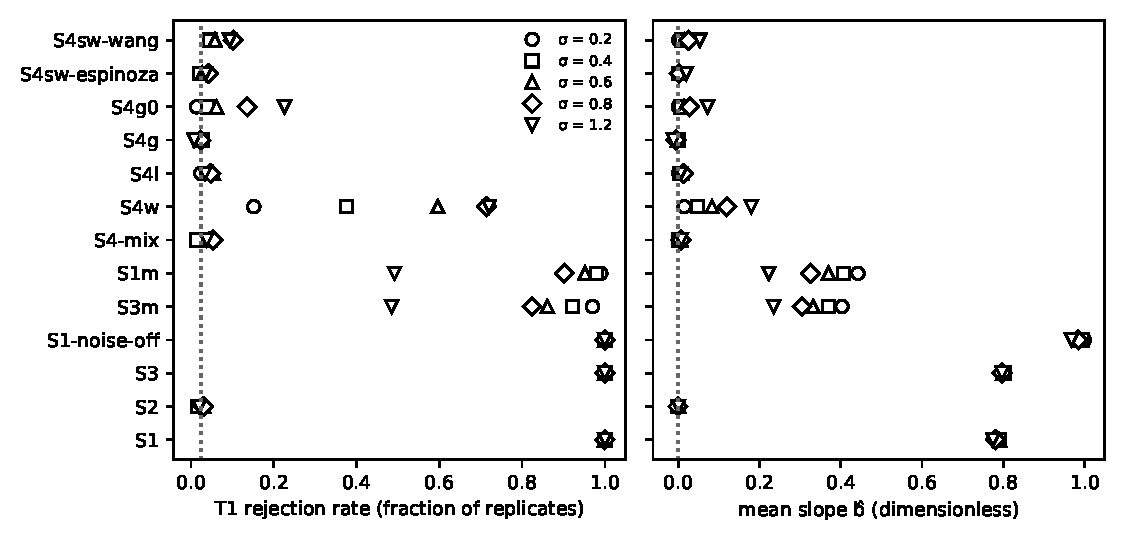
\includegraphics[width=0.82\textwidth]{F5_validation.pdf}
\caption{Validation of the frozen design. Left: fraction of replicates in
which T1 rejects; right: mean $\bhat$. Each row is a simulated population
(Section~\ref{sec:pops}) and each symbol a generating $\sigma$. The dotted
line marks the nominal level 0.025 (left) and zero slope (right).}
\label{fig:valid}
\end{figure*}

% =====================================================================
\section{Pre-registered result}\label{sec:results}
% =====================================================================
The primary fit gives $\shat=0.696$ for M2, compared with $0.787$ for M0.
Table~\ref{tab:primary} lists the quantities that decide the outcome;
Fig.~\ref{fig:lnT} shows the data pulsar by pulsar.

\begin{table*}
\centering
\caption{Pre-registered quantities and the simulated references that
decide the outcome. Intervals are 95 per cent; calibrated intervals widen
the Wald interval by the simulated-spread factor of the matching null
(1.015 for $b$, 1.050 for $d$). Percentiles of reference populations are
evaluated at the matched generating $\sigma$ of each population.}
\label{tab:primary}
\small
\begin{tabular}{@{}p{4.1cm}lll p{4.0cm}@{}}
\toprule
Quantity & Estimate & Interval & Reference & Verdict\\
\midrule
Placebo slope (M2 on $T_{k-1}$, $n=211$) & $-0.026$ & $[-0.108,\,0.056]$ &
$-0.357$ (S1m 2.5th) & not below: no artefact signature\\
$\bhat$ vs refutation bound & 0.268 & $[0.200,\,0.336]$ & 0.230 (S1m 2.5th)
& not below: no refutation\\
T1 signed root (M2 vs M0) & 7.398 & -- & 2.037 (S2 97.5th) & rejects\\
$\bhat$ vs bias-only & 0.268 & & 0.111 (S4-mix 97.5th) & exceeds\\
$\bhat$ vs model ceiling & 0.268 & & 0.926 (S1 97.5th) & below\\
$\dhat$ (T2, M4 vs M3) & $-0.257$ & $[-0.384,\,-0.130]$ & $-0.130$ (S3m
2.5th; S3: $-0.094$) & below: rejects\\
\midrule
\multicolumn{5}{l}{\textbf{Outcome: A2}, scaling supported with the
$\Delta\dot\nu$ term established. Power at the matched $\sigma$: T1 0.997,
T2 0.769.}\\
\bottomrule
\end{tabular}
\end{table*}

Applying the rules in order: the placebo slope is not below its bound, so
outcome D does not apply. $\bhat$ is not below the S1m 2.5th percentile, so
C does not apply. T1 rejects and $\bhat$ satisfies all three bounds, so A
applies. Because T2 rejects, the outcome is \textbf{A2}.

The estimate $\bhat=0.268$ lies at the 4.5th percentile of the model-true
population S1m, inside but near its lower edge. The bias-only population
reaches only 0.111. The secondary analyses agree with the primary one:
\begin{itemize}
\item the within-pulsar permutation test of $\bhat$ gives $p=1.0\times10^{-4}$
(the smallest value $10^4$ permutations allow);
\item the pooled Spearman correlation between $\ln R$ and $\ln T$ is
$0.60$ ($0.49$--$0.69$; 21 pulsars, completed intervals only);
\item the corresponding placebo correlation is $-0.09$ ($-0.25$ to
$0.07$), with permutation $p=0.55$.
\end{itemize}
Leave-one-out predictive scores (mean log score per interval) rank the
models M2 ($-6.834$), M4 ($-6.848$), M3 ($-6.859$), M0 ($-6.938$) and M1
($-7.393$; Fig.~\ref{fig:models}). The literal relation with unit slope
predicts worse than intercepts alone.

\begin{figure*}
\centering
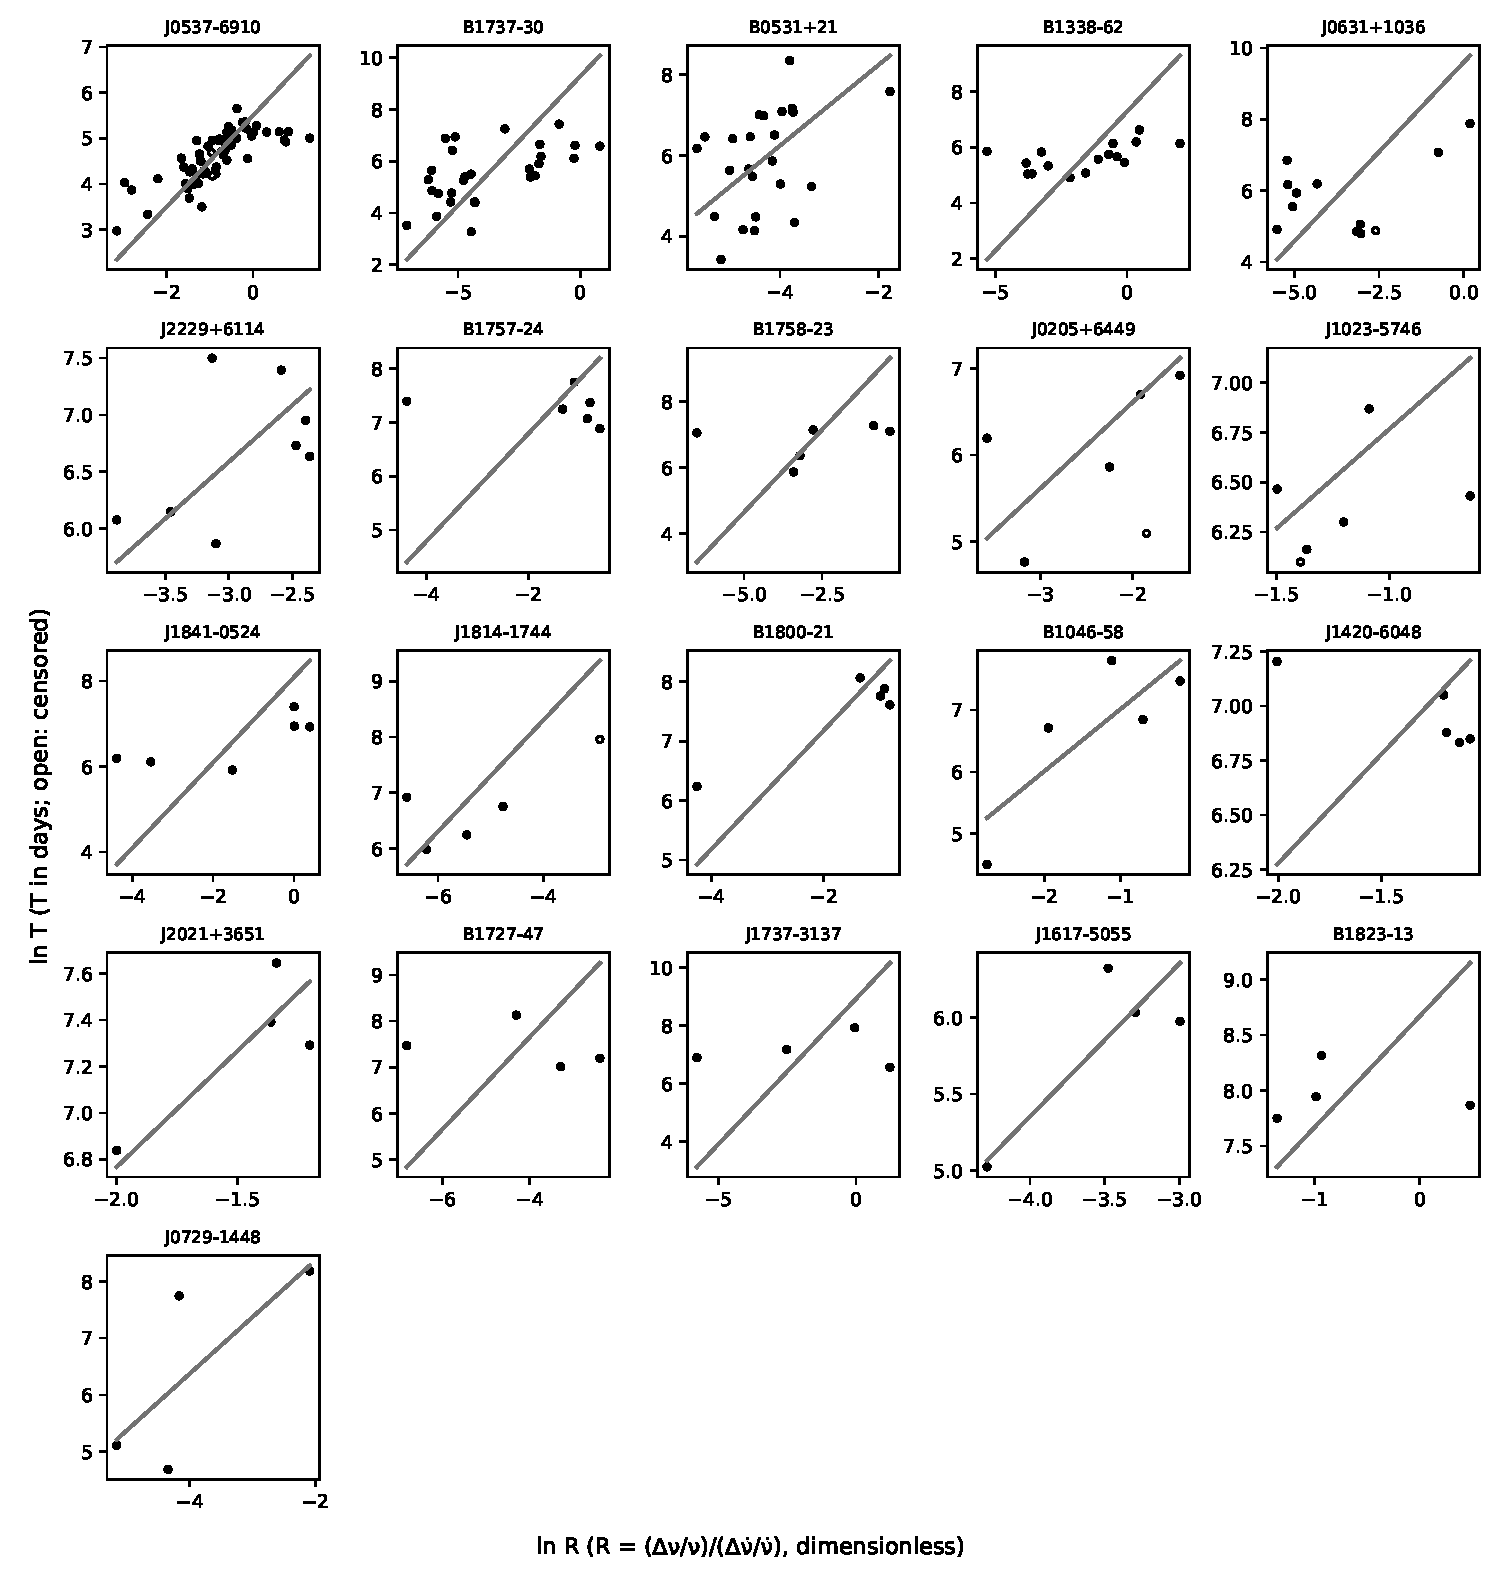
\includegraphics[width=0.92\textwidth]{F2_lnT_vs_lnR.pdf}
\caption{Waiting time against $R=(\dnu)_{-6}/(\dnud)_{-3}$ for the 21
pulsars, ordered by number of intervals. Filled symbols are completed and
open symbols censored intervals. Lines have unit slope, the literal
prediction of equation~(\ref{eq:model}); the fitted common slope is
$\bhat=0.27$.}
\label{fig:lnT}
\end{figure*}

\begin{figure}
\centering
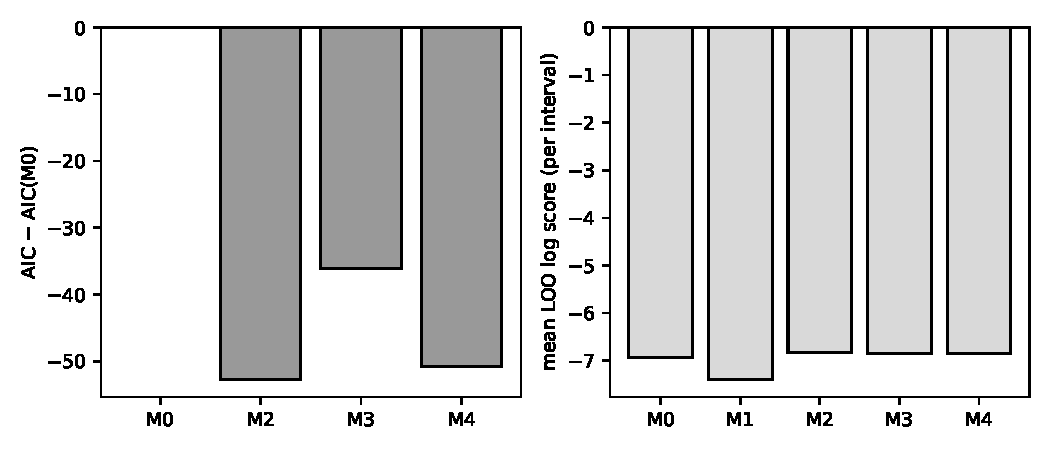
\includegraphics[width=\columnwidth]{F4_model_comparison.pdf}
\caption{Model comparison. Left: AIC relative to M0. Right: mean
leave-one-out log predictive score per interval.}
\label{fig:models}
\end{figure}

Two diagnostics complete the pre-registered set.

\emph{Missing $\Delta\dot\nu$.} Glitches without a catalogued
$\Delta\dot\nu$ tend to be followed by shorter waits (odds ratio 0.55,
0.33--0.92, $p=0.022$). Such an association is expected when a short wait
leaves too little data to measure the step. The observed log odds ratio
($-0.59$) lies inside the range produced by S1m ($-1.40$ to $-0.59$), at
its 97th percentile.

\emph{Implied $\beta$} (Table~\ref{tab:beta}; Fig.~\ref{fig:beta}). The
implied ratio is positive or consistent with zero for 20 of the 21 pulsars.
For the Crab pulsar it is $-0.47$ ($-0.48$ to $-0.45$), which is
unphysical; Section~\ref{sec:defn} traces the cause. \psr{J0537$-$6910}
gives $\beta=14.2$ (9.7--18.7).

\begin{table}
\centering
\caption{Implied $\beta_p=2\times10^{-3}\tau_{{\rm sd},p}{\rm e}^{-c_p}-
\tfrac12$ with 95 per cent intervals, from the intercepts of M1. Class is
the pre-registered D7 split (Vela-like if the median usable $\dnu\geq
10^{-6}$).}
\label{tab:beta}
\small
\footnotesize\setlength{\tabcolsep}{3pt}
\begin{tabular}{@{}lrlrrl@{}}
\toprule
Pulsar & $n$ & Class & $c_p$ & $\beta$ & 95\% interval\\
\midrule
PSR~J0537$-$6910 & 63 & Crab-like & 5.50 & 14.22 & [9.74, 18.70] \\
PSR~B1737$-$30 & 28 & Crab-like & 9.29 & 0.90 & [0.26, 1.53] \\
PSR~B0531+21 & 24 & Crab-like & 10.24 & $-$0.47 & [$-$0.48, $-$0.45] \\
PSR~B1338$-$62 & 16 & Crab-like & 7.28 & 5.59 & [1.94, 9.25] \\
PSR~J0631+1036 & 12 & Crab-like & 9.59 & 1.72 & [0.13, 3.31] \\
PSR~J2229+6114 & 8 & Crab-like & 9.59 & 0.03 & [$-$0.42, 0.48] \\
PSR~B1757$-$24 & 6 & Vela-like & 8.79 & 1.22 & [$-$0.47, 2.90] \\
PSR~B1758$-$23 & 6 & Crab-like & 9.65 & 2.26 & [$-$0.45, 4.96] \\
PSR~J0205+6449 & 6 & Vela-like & 8.61 & 0.21 & [$-$0.53, 0.96] \\
PSR~J1023$-$5746 & 6 & Vela-like & 7.77 & 0.92 & [$-$0.52, 2.37] \\
PSR~J1841$-$0524 & 6 & Crab-like & 8.09 & 6.26 & [$-$0.37, 12.89] \\
PSR~B1046$-$58 & 5 & Vela-like & 8.01 & 4.44 & [$-$0.86, 9.74] \\
PSR~B1800$-$21 & 5 & Vela-like & 9.18 & 0.68 & [$-$0.59, 1.96] \\
PSR~J1420$-$6048 & 5 & Vela-like & 8.28 & 1.91 & [$-$0.68, 4.49] \\
PSR~J1814$-$1744 & 5 & Crab-like & 12.30 & $-$0.22 & [$-$0.54, 0.10] \\
PSR~B1727$-$47 & 4 & Crab-like & 11.65 & 0.01 & [$-$0.60, 0.62] \\
PSR~B1823$-$13 & 4 & Vela-like & 8.67 & 2.18 & [$-$1.04, 5.40] \\
PSR~J0729$-$1448 & 4 & Crab-like & 10.37 & 0.31 & [$-$0.66, 1.27] \\
PSR~J1617$-$5055 & 4 & Crab-like & 9.35 & 0.02 & [$-$0.60, 0.63] \\
PSR~J1737$-$3137 & 4 & Crab-like & 8.92 & 4.53 & [$-$1.51, 10.57] \\
PSR~J2021+3651 & 4 & Vela-like & 8.77 & 1.46 & [$-$0.89, 3.80] \\
\bottomrule
\end{tabular}
\end{table}

\begin{figure}
\centering
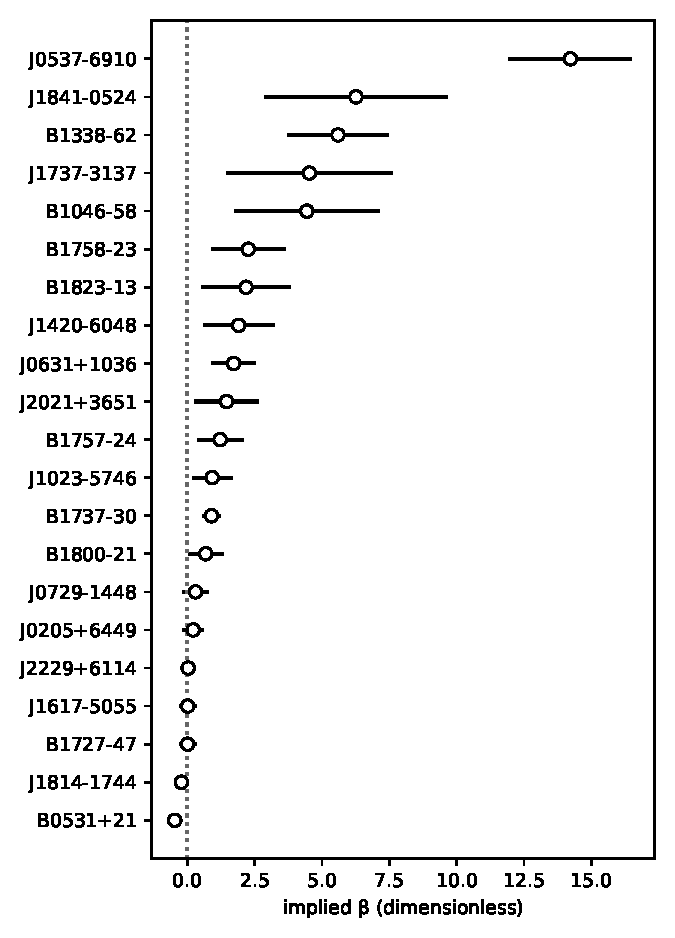
\includegraphics[width=\columnwidth]{F6_implied_beta.pdf}
\caption{Implied inertia ratio $\beta$ per pulsar with $\pm1$ standard
error bars (95 per cent intervals are given in Table~\ref{tab:beta}). The
dotted line marks $\beta=0$.}
\label{fig:beta}
\end{figure}

\subsection{Robustness}
The pre-registered robustness cases (Table~\ref{tab:robust}) receive no
outcome. Their intervals reuse the primary calibration factors and are
approximate. The slope $\bhat$ keeps its sign in every case. $\dhat$ keeps
its sign in every case except four: the global-fit class (33 intervals),
\psr{B1338$-$62} alone (16), \psr{J0631+1036} alone (12) and the
Vela-like group (41). All four intervals are wide and include zero.
The test of step-only $\Delta\dot\nu$ values could not be run, because the
catalogue does not record them.

\begin{table*}
\centering
\caption{Pre-registered robustness cases (estimates reported, no outcome
assigned). Intervals are approximate: they use the primary calibration
factors.}
\label{tab:robust}
\small
\begin{tabular}{@{}lrrlll@{}}
\toprule
Case & $n$ & Pulsars & $\bhat$ [95\%] & $\dhat$ [95\%] & $\shat$\\
\midrule
Primary & 225 & 21 & 0.268 [0.200, 0.336] & $-0.257$ [$-0.384$, $-0.130$] & 0.696\\
Without \psr{J0537$-$6910} & 162 & 20 & 0.242 [0.161, 0.323] & $-0.248$ [$-0.401$, $-0.096$] & 0.780\\
Without the Crab pulsar & 201 & 20 & 0.255 [0.194, 0.316] & $-0.208$ [$-0.327$, $-0.089$] & 0.613\\
Censored intervals dropped & 219 & 21 & 0.262 [0.194, 0.330] & $-0.240$ [$-0.369$, $-0.111$] & 0.695\\
$\sigma_{\ln R}\leq0.5$ & 156 & 15 & 0.304 [0.226, 0.382] & $-0.407$ [$-0.574$, $-0.240$] & 0.626\\
Gap-flagged intervals excluded & 224 & 21 & 0.268 [0.201, 0.336] & $-0.258$ [$-0.385$, $-0.131$] & 0.696\\
$\dnu\geq10^{-7}$ & 122 & 12 & 0.418 [0.325, 0.512] & $-0.260$ [$-0.381$, $-0.138$] & 0.402\\
Epoch uncertainty $\leq0.1\,T$ & 196 & 21 & 0.242 [0.168, 0.316] & $-0.235$ [$-0.371$, $-0.100$] & 0.702\\
Later censoring for Jodrell Bank pulsars & 231 & 21 & 0.283 [0.214, 0.353] & $-0.271$ [$-0.400$, $-0.142$] & 0.717\\
Without maintainers' own measurements & 208 & 18 & 0.280 [0.208, 0.352] & $-0.266$ [$-0.399$, $-0.133$] & 0.702\\
\midrule
Class: local relaxation & 63 & 1 & 0.480 [0.378, 0.582] & $-0.182$ [$-0.340$, $-0.024$] & 0.351\\
Class: short window & 81 & 8 & 0.213 [0.081, 0.345] & $-0.332$ [$-0.578$, $-0.086$] & 0.917\\
Class: global with exponentials & 33 & 6 & 0.128 [$-0.028$, 0.283] & $+0.269$ [$-0.114$, 0.651] & 0.498\\
Class: unknown (excluded from primary) & 28 & 3 & 0.198 [$-0.017$, 0.413] & $-0.244$ [$-0.548$, 0.059] & 0.971\\
\midrule
\psr{B0531+21} alone & 24 & 1 & 0.604 [0.028, 1.180] & $-0.740$ [$-1.442$, $-0.037$] & 1.138\\
\psr{B1737$-$30} alone & 28 & 1 & 0.279 [0.119, 0.438] & $-0.727$ [$-0.995$, $-0.459$] & 0.910\\
\psr{B1338$-$62} alone & 16 & 1 & 0.133 [0.029, 0.236] & $+0.006$ [$-0.238$, 0.250] & 0.401\\
\psr{J0631+1036} alone & 12 & 1 & 0.263 [$-0.014$, 0.539] & $+0.129$ [$-0.494$, 0.752] & 0.845\\
\midrule
D7 Crab-like (exploratory) & 184 & 13 & 0.264 [0.190, 0.338] & $-0.300$ [$-0.438$, $-0.161$] & 0.732\\
D7 Vela-like (exploratory) & 41 & 8 & 0.331 [0.148, 0.515] & $+0.294$ [$-0.072$, 0.660] & 0.499\\
\bottomrule
\end{tabular}
\end{table*}

% =====================================================================
\section{Post hoc analyses}\label{sec:posthoc}
% =====================================================================
The analyses in this section were chosen after the primary result was
known. They are not part of the pre-registration, cannot change the
outcome, and are reported to show where the result comes from.

\emph{Ratio form.} This comparison uses only the pre-registered fits of
M2 and M4, but was not itself specified in advance. M4 and M2 reach almost
the same likelihood ($\Delta\ln
L=0.026$), with $\hat a=0.268$ and $\dhat=-0.257$ in M4. The data are thus
consistent with $\dnu$ and $\dnud$ entering only through their ratio, as
equation~(\ref{eq:t0}) requires. Because measurement is expected to
attenuate $d$ more than $a$, this near-equality should not be over-read.

\emph{Intervals shorter than the fit window.} If the next glitch falls
inside a short-window fit span, the measured step and the following wait
are coupled. Four of the 100 short-window intervals are shorter than the
span. Without them $\dhat=-0.179$ ($-0.304$ to $-0.053$).

\emph{Influence.} Removing any single interval leaves $\dhat$ between
$-0.278$ and $-0.208$ (225 refits, none failed). Of the five most
influential intervals, three are short waits of \psr{B1737$-$30} (26,
34 and 48\,d; ranks 1, 2 and 5); the other two are long waits of
\psr{B1758$-$23} (1154\,d) and \psr{J2229+6114} (352.5\,d).

\emph{Single-pulsar references.} For the three pulsars with the most
intervals, each pulsar was simulated alone under S3m, under its own-method
bias-only population and under S1m, with $\sigma$ matched to its own M4
fit (Table~\ref{tab:single}).
\begin{itemize}
\item In \psr{B1737$-$30} and \psr{J0537$-$6910}, which are measured by
different methods, $\dhat$ lies beyond the size-only and bias-only ranges
and within the model-true range.
\item For the Crab pulsar all three ranges are so wide that the test is
uninformative.
\end{itemize}

\begin{table}
\centering
\caption{Post hoc single-pulsar test of $\dhat$: percentile of the observed
value within each simulated population (1000 replicates), with the
population's 95 per cent range in brackets.}
\label{tab:single}
\small
\footnotesize\setlength{\tabcolsep}{3pt}
\begin{tabular}{@{}lccc@{}}
\toprule
 & \psr{B1737$-$30} & \psr{J0537$-$6910} & \psr{B0531+21}\\
\midrule
Method & SW & LR & SW\\
$\dhat$ (own M4) & $-0.727$ & $-0.182$ & $-0.740$\\
$\shat$ (own M4) & 0.73 & 0.30 & 1.13\\
\midrule
\multirow{2}{*}{S3m} & 0.1 & 0.3 & 8.4\\
 & {\scriptsize[$-0.31$, 0.34]} & {\scriptsize[$-0.13$, 0.13]} & {\scriptsize[$-1.15$, 1.03]}\\
\multirow{2}{*}{Own bias} & 0.0 & 0.5 & 11.3\\
 & {\scriptsize[$-0.36$, 0.34]} & {\scriptsize[$-0.14$, 0.11]} & {\scriptsize[$-1.43$, 1.29]}\\
\multirow{2}{*}{S1m} & 9.5 & 32.6 & 9.8\\
 & {\scriptsize[$-1.30$, 1.18]} & {\scriptsize[$-0.38$, 0.12]} & {\scriptsize[$-1.58$, 1.12]}\\
\bottomrule
\end{tabular}
\end{table}

\emph{Heterogeneity.} For the 11 pulsars with at least six intervals (181
intervals), M4 with a separate size coefficient per pulsar was compared with
and without a separate $d$ per pulsar. The likelihood ratio is $28.2$ for
10 degrees of freedom ($p=0.0017$), with common $\dhat=-0.41\pm0.07$.
\begin{itemize}
\item \psr{B1737$-$30} ($-0.73\pm0.11$) and the Crab pulsar ($-0.74\pm0.18$)
show a strong effect.
\item \psr{J0537$-$6910} ($-0.18\pm0.15$) shows a weak one.
\item \psr{B1338$-$62} ($+0.01\pm0.19$) and \psr{J0631+1036} ($+0.13\pm
0.23$) show none.
\end{itemize}
The nominal $p$-value overstates the evidence for two reasons. The model
forces a common $\sigma$ on pulsars whose single-pulsar fits range from
$\shat=0.30$ to 1.13. And different method mixes are expected to attenuate
the measured $d$ by different amounts even if the true $d$ were universal.

% =====================================================================
\section{Discussion}\label{sec:disc}
% =====================================================================
\subsection{What the result does and does not show}
Under rules fixed in advance, within-pulsar waiting times scale with the
creep ratio $R$. The spin-down step carries the predicted negative sign at
fixed glitch size, beyond what glitch size alone or the emulated measurement
biases produce. That is the creep-specific content of
equation~(\ref{eq:t0}), and the outcome is the strongest the design
allowed.

The result does not establish the relation quantitatively. The slope is
far below unity and M1 predicts worse than intercepts alone. The emulation
attributes the shortfall to attenuation by $\Delta\dot\nu$ measurement, but
$\bhat$ sits at the 4.5th percentile of the emulated model-true population,
and the real $\shat=0.696$ is below the emulated floor of about 0.74. Both
suggest that the emulation degrades $\Delta\dot\nu$ somewhat more than real
measurements do. The verdict is relative to that emulation: a more faithful
one could move the reference ranges.

\subsection{Which \texorpdfstring{$\Delta\dot\nu$}{spin-down step}?}\label{sec:defn}
Equation~(\ref{eq:steps}) refers to the step that persists after the prompt
transients. The catalogue mixes that quantity with instantaneous totals
(global fits) and with short-window differences that average the transients
over 30--50\,d \citep{espinoza2011}.

The Crab pulsar shows how much this matters. Its catalogue $\dnud$ values
in the primary sample are a median of 16 (range 1.1--53) times the
persistent step implied by $|\Delta\dot\nu_{\rm p}|\approx7\times10^{-8}\,
\Delta\nu$ \citep{lyne2015}, because its recoveries are large ($Q\sim0.6$--1)
and fast \citep{wong2001,wang2012}.
\begin{itemize}
\item Replacing the catalogue values with that persistent step moves the
Crab's implied $\beta$ from $-0.47$ to $-0.04$.
\item Counting only the 54 per cent of the step that appears promptly
\citep{lyne2015} gives $+0.34$.
\end{itemize}
The negative $\beta$ is therefore a definitional artefact. Because a
constant factor is absorbed by the per-pulsar intercept, it leaves the
within-pulsar slopes untouched. This check was made after the freeze, uses an
average scaling rather than per-glitch persistent steps, and is reproduced
by \texttt{scripts/posthoc\_crab\_persistent\_step.py} in the repository.

By contrast, \psr{J0537$-$6910} is measured as a persistent step
\citep{antonopoulou2018}, matching the definition of Eq.~(\ref{eq:steps}).
Its $\beta\approx14$ implies, with typical $\dnud\sim0.5\times10^{-3}$,
$I_{\rm B}/I\approx1$ per cent, which is plausible for a crustal superfluid
reservoir.

The two pulsars without a $\Delta\dot\nu$ effect may also be measurement
cases, though this is an untested hypothesis. Most glitches of
\psr{J0631+1036} are tiny ($\dnu$ of 0.4--43$\times10^{-9}$), and three of its
catalogue $\dnud$ values are negative; a step near the short-window
detection floor would attenuate $d$ towards zero. Across its 16 primary
intervals, \psr{B1338$-$62}'s $\dnud$ spans 0.20--5.00$\times10^{-3}$
while its $\dnu$ spans a factor of about 700; for its seven global-fit
glitches alone \citep{lower2021}, $\dnud$ spans only
0.22--1.06$\times10^{-3}$ over the same factor of about 700 in $\dnu$. That could reflect a similar floor, or small glitches
that are not creep-cycle events.

There is a tension here worth stating plainly. \citet{zhou2022} expect
equation~(\ref{eq:t0}) to work best for Vela-like glitches, yet the
effect is clearest in two frequent, small-glitch pulsars measured by short
windows, and the exploratory Vela-like group gives a positive $\dhat$.

\subsection{The Vela pulsar}\label{sec:vela}
Vela would be a natural out-of-sample test, but it cannot be used with the
catalogue values. For its 16 usable glitches with
$\dnu\geq10^{-6}$, the catalogued $\dnud$ ranges from about $6$ to
$600\times10^{-3}$, depending on the source:
\begin{itemize}
\item several values come from hours of data immediately after the glitch
(e.g.\ the HartRAO reports of the 2010 and 2013 glitches used 14 and 9\,h of
data), and so are dominated by the fastest transients;
\item a few, such as the four-component fit of the 2000 glitch with
$\dnud\approx6.7\times10^{-3}$ \citep{dodson2002}, are comparable with
Eq.~(\ref{eq:steps}).
\end{itemize}
Only one of Vela's usable glitches has an audited, admissible
measurement, far below the four admissible intervals the rules require. A uniform re-measurement of Vela's persistent steps from timing
data would allow a direct test.

\subsection{Limitations}
\begin{enumerate}
\item \emph{Shared scatter.} The primary model uses one $\sigma$ for all
pulsars, which the single-pulsar fits contradict. The simulations share the
assumption, so calibration does not correct for it. A hierarchical model
with pulsar-specific scatter and partially pooled slopes would be the
natural next step.
\item \emph{Emulation.} See Section~\ref{sec:emullimits}: no
phase-connected fitting, no red noise, two uncited settings, and four to
six pulsars, depending on $\sigma$, whose emulated uncertainties exceed
the catalogue's.
\item \emph{Sample.} \psr{J0537$-$6910} contributes 28 per cent of the
intervals, though the result survives its removal. The method behind the
catalogue maintainers' own measurements is assumed (robustness case
included).
\item \emph{Constant $\beta$.} Equation~(\ref{eq:model}) assumes $\beta_p$
is constant within a pulsar.
\item \emph{Self-held pre-registration.} The freeze is attested by the
author's version-control history and an e-mailed record of the checksums, not
by a public registry. The rules were
amended sixteen times before the freeze, partly in response to simulated
power.
\end{enumerate}

\subsection{A forward test}
To obtain evidence that cannot have been tuned after the fact, I fixed on
2026 November 12, using the frozen M2 and M0 fits, forecasts of the next
glitch for six pulsars. These pulsars are monitored by Jodrell Bank, have
no documented end of monitoring, and have a current glitch-free stretch no
longer than their longest catalogued wait. The forecasts will be scored on
2028 November 1 by the difference in log predictive density between M2
and M0 (Appendix~\ref{app:forecast}). With six pulsars and windows spanning
years, this is a weak test, but an honest one.

% =====================================================================
\section{Conclusions}\label{sec:concl}
% =====================================================================
A pre-registered test of the vortex-creep waiting-time relation
(\citealt{zhou2022}, equation~48), run once on 225 intervals in 21 pulsars
and calibrated against emulations of the methods that produced the
catalogue's $\Delta\dot\nu$, supports both its scaling and its
creep-specific spin-down dependence.

The support is qualitative. The slope is strongly attenuated, the
spin-down dependence varies between pulsars, and the sign of the effect is
best established in \psr{B1737$-$30} and \psr{J0537$-$6910}. The largest
remaining uncertainty is the definition of $\Delta\dot\nu$:
equation~(\ref{eq:t0}) needs the persistent step, while most catalogue
values include transients. A uniform measurement of persistent steps would
turn this qualitative test into a quantitative one.

\section*{Acknowledgements}
I thank the maintainers of the Jodrell Bank Glitch Catalogue and the ATNF
Pulsar Catalogue for making their data public. This work made use of
\textsc{numpy}, \textsc{scipy}, \textsc{pandas}, \textsc{matplotlib} and
\textsc{lifelines}. An AI assistant, Claude Opus~5.5 \citep{anthropic2026},
used through Claude Code, contributed to the development of the analysis
rules and pre-freeze amendments (D4a--D4p), wrote the analysis code under
the author's instructions, reviewed computational results, checked the D4o
recovery parameters against the cited literature, and assisted in drafting
and revising the manuscript and in checking its statements against the
analysis repository. The author directed the research, critically evaluated
the work, and takes full responsibility for the paper. No AI tool is an
author; the assistant's contributions are documented in the analysis
repository.

\section*{Data Availability}
The glitch data are public in the Jodrell Bank Glitch Catalogue. The
analysis repository,
\url{https://github.com/deeyanbothra10-droid/glitch-waiting-time-v2}, is
available from the author on request. It contains the code, the catalogue snapshot used (distributed under the
catalogue's own terms), the frozen rules and their checksum records, the
results and figures, the forecast files, and a guide to verifying the
checksums of Section~\ref{sec:prereg}.

% =====================================================================
\bibliographystyle{mnras}
\begin{thebibliography}{99}
\bibitem[\protect\citeauthoryear{Akbal et al.}{2017}]{akbal2017}
Akbal O., Alpar M.~A., Buchner S., Pines D., 2017, \mnrasref{469}{4183}
(doi:10.1093/mnras/stx1095)

\bibitem[\protect\citeauthoryear{Akbal, G\"ugercino\u{g}lu \& Alpar}{2021}]{akbal2021}
Akbal O., G\"ugercino\u{g}lu E., Alpar M.~A., 2021, preprint
(arXiv:2106.03341)

\bibitem[\protect\citeauthoryear{Alpar et al.}{1984}]{alpar1984}
Alpar M.~A., Anderson P.~W., Pines D., Shaham J., 1984, ApJ, 276, 325

\bibitem[\protect\citeauthoryear{Alpar \& Baykal}{2006}]{alpar2006}
Alpar M.~A., Baykal A., 2006, \mnrasref{372}{489}

\bibitem[\protect\citeauthoryear{Anderson \& Itoh}{1975}]{anderson1975}
Anderson P.~W., Itoh N., 1975, Nature, 256, 25

\bibitem[\protect\citeauthoryear{Anthropic}{2026}]{anthropic2026}
Anthropic, 2026, Claude Opus 5.5, large language model (model ID
claude-opus-5-5), used through Claude Code from 2026 October 31 to
November 13, \url{https://platform.claude.com/docs/en/models/opus-5-5/overview}

\bibitem[\protect\citeauthoryear{Antonopoulou et al.}{2018}]{antonopoulou2018}
Antonopoulou D., Espinoza C.~M., Kuiper L., Andersson N., 2018,
\mnrasref{473}{1644} (doi:10.1093/mnras/stx2429)

\bibitem[\protect\citeauthoryear{Antonopoulou, Haskell \& Espinoza}{2022}]{antonopoulou2022}
Antonopoulou D., Haskell B., Espinoza C.~M., 2022, Rep. Prog. Phys., 85,
126901

\bibitem[\protect\citeauthoryear{Basu et al.}{2022}]{basu2022}
Basu A., et al., 2022, \mnrasref{510}{4049} (doi:10.1093/mnras/stab3336)

\bibitem[\protect\citeauthoryear{Davidson-Pilon}{2019}]{davidson2019}
Davidson-Pilon C., 2019, J. Open Source Softw., 4, 1317

\bibitem[\protect\citeauthoryear{Dodson, McCulloch \& Lewis}{2002}]{dodson2002}
Dodson R.~G., McCulloch P.~M., Lewis D.~R., 2002, ApJ, 564, L85
(doi:10.1086/339068)

\bibitem[\protect\citeauthoryear{Espinoza et al.}{2011}]{espinoza2011}
Espinoza C.~M., Lyne A.~G., Stappers B.~W., Kramer M., 2011,
\mnrasref{414}{1679} (doi:10.1111/j.1365-2966.2011.18503.x)

\bibitem[\protect\citeauthoryear{G\"ugercino\u{g}lu \& Alpar}{2020}]{gugercinoglu2020}
G\"ugercino\u{g}lu E., Alpar M.~A., 2020, \mnrasref{496}{2506}
(doi:10.1093/mnras/staa1672)

\bibitem[\protect\citeauthoryear{G\"ugercino\u{g}lu et al.}{2022}]{gugercinoglu2022}
G\"ugercino\u{g}lu E., Ge M.~Y., Yuan J.~P., Zhou S.~Q., 2022,
\mnrasref{511}{425} (doi:10.1093/mnras/stac026)

\bibitem[\protect\citeauthoryear{Haskell \& Melatos}{2015}]{haskell2015}
Haskell B., Melatos A., 2015, Int. J. Mod. Phys. D, 24, 1530008

\bibitem[\protect\citeauthoryear{Ho et al.}{2026}]{ho2026}
Ho W.~C.~G., et al., 2026, MNRAS, in press (doi:10.1093/mnras/staf2264;
arXiv:2512.19800)

\bibitem[\protect\citeauthoryear{Lower et al.}{2021}]{lower2021}
Lower M.~E., et al., 2021, \mnrasref{508}{3251} (doi:10.1093/mnras/stab2678)

\bibitem[\protect\citeauthoryear{Lyne et al.}{2015}]{lyne2015}
Lyne A.~G., Jordan C.~A., Graham-Smith F., Espinoza C.~M., Stappers B.~W.,
Weltevrede P., 2015, \mnrasref{446}{857} (doi:10.1093/mnras/stu2118)

\bibitem[\protect\citeauthoryear{Manchester et al.}{2005}]{manchester2005}
Manchester R.~N., Hobbs G.~B., Teoh A., Hobbs M., 2005, AJ, 129, 1993

\bibitem[\protect\citeauthoryear{Middleditch et al.}{2006}]{middleditch2006}
Middleditch J., Marshall F.~E., Wang Q.~D., Gotthelf E.~V., Zhang W., 2006,
ApJ, 652, 1531 (doi:10.1086/508736)

\bibitem[\protect\citeauthoryear{Wang et al.}{2000}]{wang2000}
Wang N., Manchester R.~N., Pace R.~T., Bailes M., Kaspi V.~M., Stappers
B.~W., Lyne A.~G., 2000, \mnrasref{317}{843}
(doi:10.1046/j.1365-8711.2000.03713.x)

\bibitem[\protect\citeauthoryear{Wang et al.}{2012}]{wang2012}
Wang J., Wang N., Tong H., Yuan J., 2012, Ap\&SS, 340, 307
(doi:10.1007/s10509-012-1058-x)

\bibitem[\protect\citeauthoryear{Wong, Backer \& Lyne}{2001}]{wong2001}
Wong T., Backer D.~C., Lyne A.~G., 2001, ApJ, 548, 447 (doi:10.1086/318657)

\bibitem[\protect\citeauthoryear{Yu et al.}{2013}]{yu2013}
Yu M., et al., 2013, \mnrasref{429}{688}

\bibitem[\protect\citeauthoryear{Zhou et al.}{2022}]{zhou2022}
Zhou S., G\"ugercino\u{g}lu E., Yuan J., Ge M., Yu C., 2022, Universe, 8,
641 (doi:10.3390/universe8120641)

\bibitem[\protect\citeauthoryear{Zubieta et al.}{2026}]{zubieta2026}
Zubieta E., Espinoza C.~M., Antonopoulou D., Ho W.~C.~G., Kuiper L.,
Garc\'ia F., del Palacio S., 2026, A\&A, 706, A61
(doi:10.1051/0004-6361/202557555)
\end{thebibliography}

% =====================================================================
\appendix
\section{Pre-freeze amendments}\label{app:amend}
% =====================================================================
Table~\ref{tab:amend} lists the amendments to the original rules (D1--D15,
2026 October 31). Every one was recorded in the decision file before the
freeze; eleven state their reason explicitly, while D4b and D4d--D4g do
not. None was made after a statistic relating glitch
properties to real waiting times had been computed. ``Prompted by
simulation'' marks amendments motivated by simulated power, error rates or
emulator behaviour. This column is the author's classification, based on
the stated reasons where they are given, not a field recorded in the
decision file.

\begin{table*}
\centering
\caption{Amendments to the analysis rules before the freeze.}
\label{tab:amend}
\small
\begin{tabular}{@{}llp{11.2cm}c@{}}
\toprule
ID & Date & Change & Prompted by simulation\\
\midrule
D4a & Oct 31 & Permutation, Spearman and leave-one-out details & no\\
D4b & Oct 31 & Interval conventions; simulation centring; validation cost limits; conditional-logit missingness check & no\\
D4c & Oct 31 & Two simulation layers (S1--S3 statistics only; S1m and S4 through the emulation); emulation settings & yes (emulator behaviour)\\
D4d & Oct 31 & S4 treated as measurement, not test; AIC rule for exponentials; decision rules calibrated against S1m and S4-mix & yes\\
D4e & Oct 31 & Noise calibration to formal uncertainties; replicate inclusion rule & yes\\
D4f & Oct 31 & Short-window class created from the source audit, with a fixed admission rule & no (audit)\\
D4g & Oct 31 & Documented censoring dates; RXTE/NICER gap of \psr{J0537$-$6910}; Jodrell Bank robustness case & no (audit)\\
D4h & Oct 31 & Intercepts corrected for covariate spread; false-positive bound tied to $\alpha=0.025$ & yes\\
D4i & Oct 31 & Tiered outcomes; implied $\beta$ made report-only & yes (power)\\
D4j & Oct 31 & Exclusive outcome order; artefact outcome redefined so that a null result is not labelled an artefact & yes\\
D4k & Oct 31 & Failed-replicate rule; $\sigma$ grid extended to 0.8 and 1.2 & yes\\
D4l & Nov 1 & Directional, simulation-calibrated T1 and T2; corrected bounds for C and A & yes (error rates)\\
D4m & Nov 1 & Measured size-only null S3m; A1 relabelled as not specific to creep; calibrated intervals & yes\\
D4n & Nov 1 & Generating $\sigma$ matched to fitted scatter; T2 based on $\dhat$ against null references & yes (power)\\
D4o & Nov 1 & Literature-based recovery parameters replace placeholders & no (literature)\\
D4p & Nov 1 & Search bounds, robustness reporting, outcome labels, removal of provisional tags & no\\
\bottomrule
\end{tabular}
\end{table*}

% =====================================================================
\section{Source audit}\label{app:audit}
% =====================================================================
\begin{table*}
\centering
\caption{Audited sources of admissible $\Delta\dot\nu$ values. $N$ is the
glitch count recorded for each source in the project's source-audit file
(\texttt{data/meta/source\_audit.csv}); it is a bookkeeping count from the
audit worklist, not a count of catalogue entries, and its derivation was not
recorded. ``Our
measurement'' denotes the catalogue maintainers' own values, whose method
is assumed to follow \citet{basu2022}.}
\label{tab:audit}
\small
\begin{tabular}{@{}lrlllp{6.2cm}@{}}
\toprule
Source & $N$ & Telescope & Cadence (d) & Class & $\Delta\dot\nu$ as reported\\
\midrule
\citet{espinoza2011} & 103 & Lovell & 2--10 & short window & difference of pre- and post-glitch solutions at the epoch; post-glitch span ideally 30--50\,d; transients not separated\\
\citet{wang2000} & 15 & Parkes & 14--42 & short window & pre- and post-glitch solutions over $\sim$100--300\,d, extrapolated to the epoch\\
\citet{antonopoulou2018} & 45 & RXTE & $<$14 & local relaxation & persistent step; fits bounded by neighbouring glitches\\
\citet{ho2026} & 23 & NICER & variable & local relaxation & glitch model fitted per segment; recovery terms where detected\\
\citet{yu2013} & 17 & Parkes & 14--28 & local relaxation & segment fits centred on the glitch; recoveries where detected\\
\citet{basu2022} & 36 & Lovell & 10--14 & global & $\Delta\dot\nu_{\rm p}+\sum\Delta\nu_{\rm d}/\tau_{\rm d}$; all glitches fitted simultaneously\\
\citet{lower2021} & 20 & Parkes & $\sim$30 & global & glitch and red-noise parameters fitted together; recoveries free\\
\citet{gugercinoglu2022} & 8 & \textit{Fermi}-LAT & 1--30 & global & spin and glitch parameters fitted together, with exponentials\\
Our measurement & 17 & Lovell & 10--14 & global (assumed) & method not published\\
\bottomrule
\end{tabular}
\end{table*}

% =====================================================================
\section{Forward forecast}\label{app:forecast}
% =====================================================================
The forecast was fixed on 2026 November 12 (SHA-256 of the forecast file
\texttt{9f46b894\ldots f43f0}). Two earlier drafts were superseded before
any outcome could be known, because they assumed continuous monitoring for
pulsars where that was not documented. They remain in the repository.

For each scored pulsar, the wait after its last catalogued glitch $g$ is
forecast as $\ln T\sim\mathcal N(\mu,\shat^2)$ from the frozen fits (M2:
$\mu=c_p+\bhat\ln R_g$; M0: $\mu=c_p$), conditioned on no glitch before
the catalogue snapshot (MJD 61343). On 2028 November 1 the catalogue will be
downloaded again.
\begin{itemize}
\item The score is the summed log predictive density of the next glitch
under M2 minus that under M0. A pulsar with no glitch by then contributes
its log survival probability.
\item A pulsar whose next glitch turns out to predate the snapshot is void.
\end{itemize}

\begin{table}
\centering
\caption{Scored forecasts: median and central 50 per cent window of the
next-glitch date under M2 and M0.}
\label{tab:forecast}
\small
\footnotesize\setlength{\tabcolsep}{2.5pt}
\begin{tabular}{@{}llll@{}}
\toprule
Pulsar & Model & Median & 50\% window\\
\midrule
\psr{B0531+21} & M2 & 2027 May 26 & 2027 Jan 23 -- 2028 Jan 04\\
 & M0 & 2027 Jul 18 & 2027 Feb 12 -- 2028 May 05\\
\psr{J2229+6114} & M2 & 2028 Jul 31 & 2027 Sep 13 -- 2030 Jan 08\\
 & M0 & 2028 Jun 04 & 2027 Jul 23 -- 2029 Dec 09\\
\psr{J1737$-$3137} & M2 & 2028 Dec 08 & 2027 Sep 11 -- 2031 Mar 08\\
 & M0 & 2029 Apr 20 & 2027 Oct 30 -- 2032 Jan 23\\
\psr{J2021+3651} & M2 & 2029 Oct 04 & 2028 Feb 08 -- 2032 Aug 06\\
 & M0 & 2029 Aug 09 & 2027 Dec 25 -- 2032 Jul 28\\
\psr{B1800$-$21} & M2 & 2030 Nov 23 & 2028 Jul 08 -- 2035 Feb 19\\
 & M0 & 2030 Jun 21 & 2028 Apr 18 -- 2034 Jul 20\\
\psr{B1823$-$13} & M2 & 2031 May 17 & 2028 Sep 22 -- 2036 Jan 26\\
 & M0 & 2032 Apr 24 & 2029 Jan 29 -- 2038 Apr 13\\
\bottomrule
\end{tabular}
\end{table}

\begin{figure}
\centering
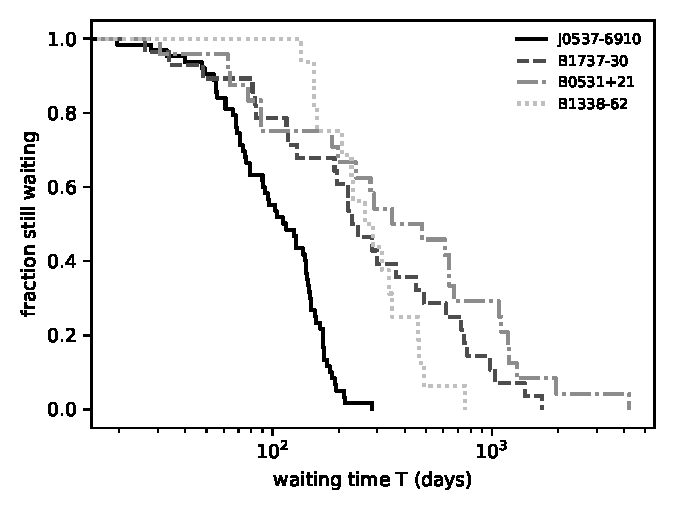
\includegraphics[width=\columnwidth]{F3_kaplan_meier.pdf}
\caption{Kaplan--Meier estimates of the fraction of intervals still waiting,
for the four pulsars with the most intervals.}
\label{fig:km}
\end{figure}

\ifmnras\label{lastpage}\fi
\end{document}
